\chapter{Ergebnisse}
In diesem Kapitel werden die Ergebnisse vorgestellt, die mithilfe den Implementierungen von L-Systemen und dem Space-Colonization Algorithmus produziert werden können.

Bei der Erstellung der Abbildungen wurden die Beleuchtungsberechnungen des Grafiksystems der Unreal Engine aktiviert.
\section{L-System-Akteur}
L-Systeme ermöglichen es mithilfe bestimmter Produktionsregeln Baumstrukturen zu generieren. Um Regeln zu finden, die realitätsnahe Ergebnisse liefern kann das Abzweigungsverhalten von biologischen Bäumen betrachtet werden.
\subsection{Monopodial}
Ein biologischer Baum mit monopodialem Abzweigungsverhalten bildet einen Hauptstamm, der stets weiterwächst, mit davon abzweigenden Nebenästen. \cite[S.21]{Forstbonatik:17} Ein Beispiel für ein solches Wachstum ist das folgende L-System:

\begin{equation}
\begin{array}{llll}
\omega & : F(100)A(100) \\
p_1 & : A(l) &\rightarrow& F(l)\text{ }[\&(a1)\text{ }B(l)]\text{ }/(d1)\text{ }A(l*r1) \\
p_2 &  : B(l) &\rightarrow& F(l)\text{ }[-(a2)\text{ }B(l*r2)]\text{ }/(d2)\text{ }B(l*r2)
\end{array}
\label{eq:ProdMonopodial}
\end{equation} 

Die Produktionsregel $p_1$ produziert den Hauptstamm, welcher in jeder Ableitung verlängert wird und einen Nebenast produziert, der anhand von $p_2$ ebenfalls entlang einer Hauptachse weiterwächst und weitere Nebenäste produziert. $a_1$ und $a_2$ entsprechen den Abzweigungswinkel neuer Äste von der Hauptachse, während die Winkel $d_1$ und $d_2$ die Rotation um die Hauptachse beschreiben, bevor ein neuer Nebenast produziert wird. $r_1$ und $r_2$ entsprechen Faktoren, welche das Wachstum eines Astes pro Ableitung verkürzen, falls der Wert unter $1$ liegt und verlängern, falls der Wert über $1$ liegt.

Abbildung \ref{fig:Monopodial}

\begin{figure} [hbtp]
	\centering
	\begin{subfigure}[t]{.7\textwidth}
		\centering
		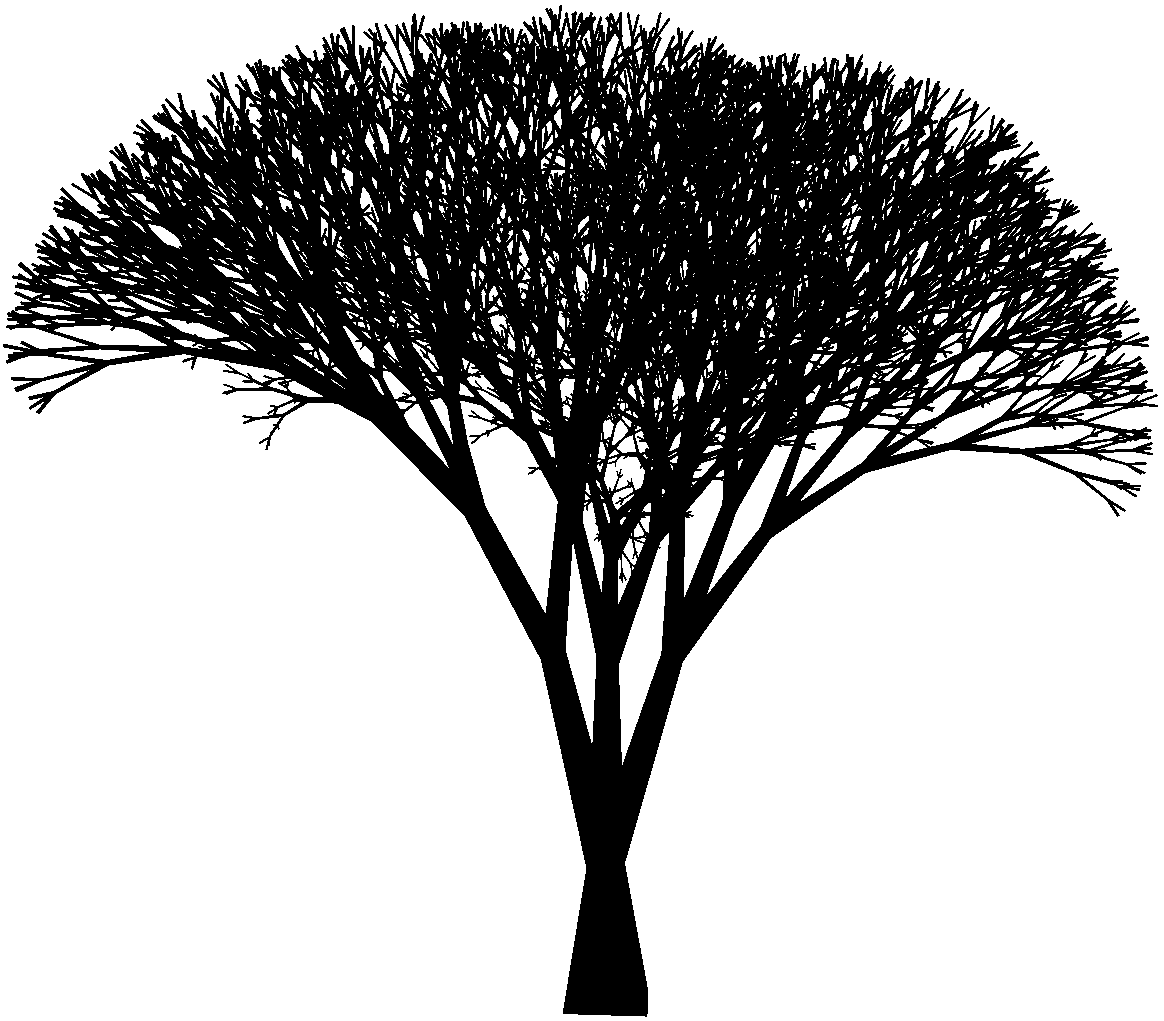
\includegraphics[width=\linewidth]{images/3DTreeP61B_Angle_18_95.png}
		\caption{$n=8$, $d=137.5\degree$, $a=18.95\degree$, $l_r=1.3$}
		\label{subfig:3DTreeP61B_Angle_18_95}
	\end{subfigure}
	\begin{subfigure}[t]{.7\textwidth}
		\centering
		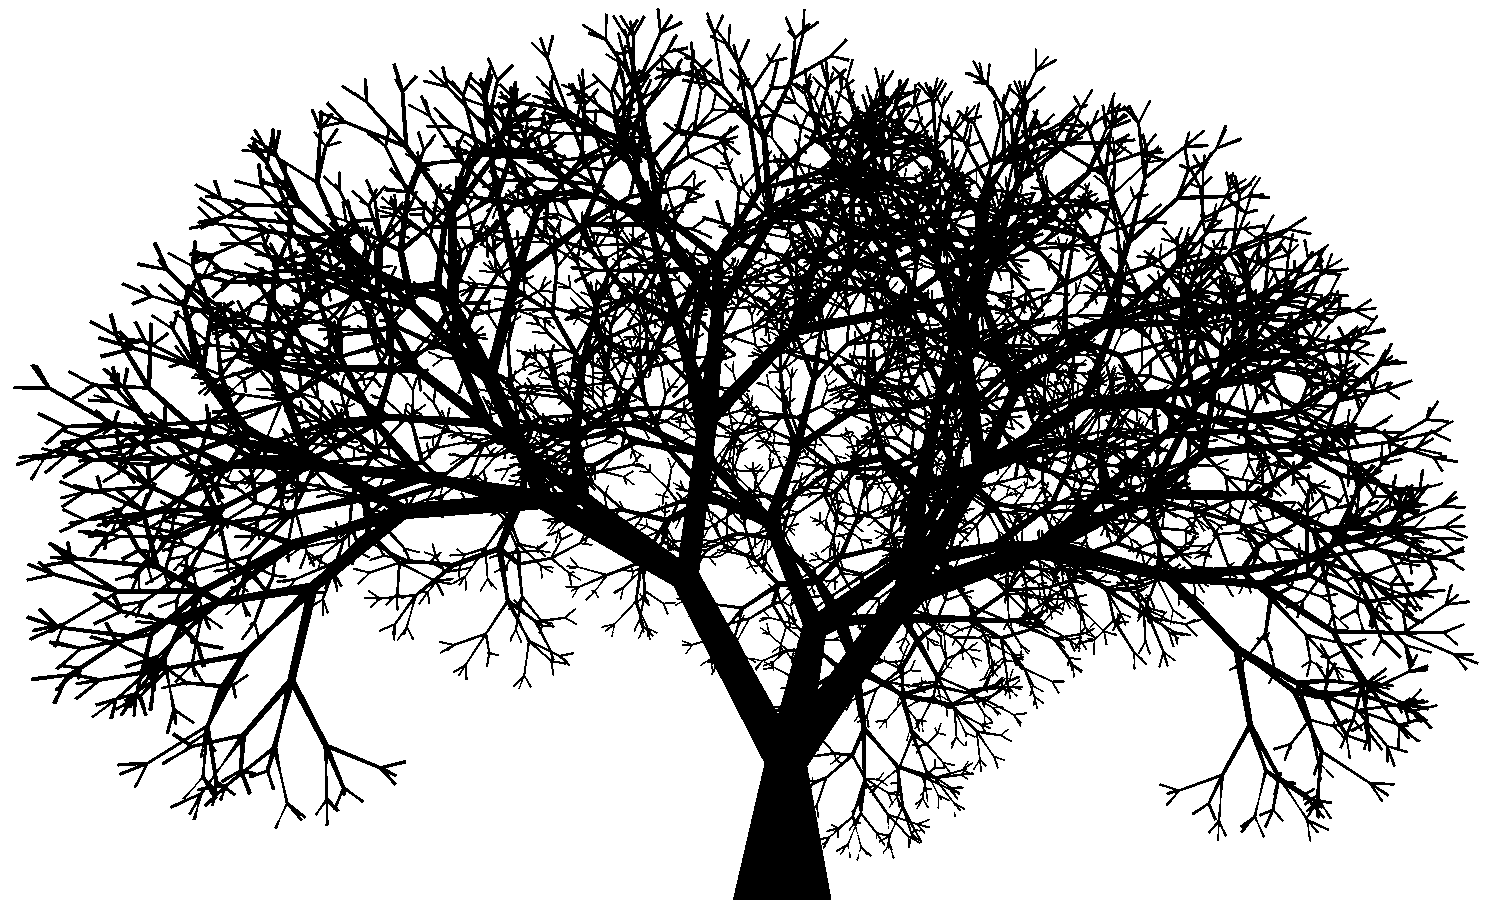
\includegraphics[width=\linewidth]{images/3DTreeP61B_Angle_36.png}
		\caption{$n=8$, $d=137.5\degree$, $a=36.0\degree$, $l_r=1.3$}
		\label{subfig:3DTreeP61B_Angle_36}
	\end{subfigure}
	\caption{Die n-fache Ableitung des Axioms anhand der Produktionsregeln aus Gleichung \ref{eq:ProdMonopodial}, visualisiert mithilfe der implementierten Turtle-Interpretation. Eigene Abbildungen.}
	\label{fig:Monopodial}
\end{figure}

\subsection{Sympodial}
Beim sympodialen Wachstum bildet ein Ast Abzweigungen, ohne selbst weiter zu wachsen. 

\begin{equation}
\begin{array}{llll}
\omega & : F(100)A(150) \\
p_1 & : A(l) &\rightarrow& F(l)\text{ }[\&(a1)\text{ }B(l*r1)]\text{ }/(180)\text{ }[\&(a2)\text{ }B(l*r2)] \\
p_2 &  : B(l) &\rightarrow& F(l)\text{ }[+(a1)\text{ }/(d1)\text{ }B(l*r1)]\text{ }[-(a2)\text{ }\backslash(d2)\text{ }B(l*r2)]
\end{array}
\label{eq:ProdMonopodial}
\end{equation} 

\subsection{Ternäre Verzweigungen}
test
\subsection{Tropismus}
Die Wahl eines Tropismusvektors erweitert diese Regeln und ermöglicht
\section{Space-Colonization-Akteur}
test
\subsection{Ursprüngliche Parameter}
test
\subsection{Erweiterte Parameter}
test

\subsection{Probleme}
Mit SCA: Gleicher Abstand von zwei Einflusspunkten führt zu beinahe unendlicher Hin- und Her-Generierung von Branches.
\\
SCA: Random-Verteilung der Punkte.

\section{Performanz}


